\documentclass[runningheads]{llncs}
\usepackage{graphicx}
\usepackage{amsmath,amssymb} % define this before the line numbering.
\usepackage{ruler}
\usepackage{color}
\usepackage{footnote}
\usepackage{multirow} 
\usepackage{cite}
\usepackage[draft]{hyperref}
\usepackage{balance}
\usepackage{subcaption}
\usepackage{algpseudocode}
\usepackage{algorithm}
\usepackage{amssymb}
\usepackage{bbm}
\usepackage[T1]{fontenc}
\usepackage[utf8]{inputenc}
%\usepackage{authblk}
\pdfminorversion=4
\DeclareMathOperator*{\argmax}{arg\,max}
\DeclareMathOperator*{\argmin}{arg\,min}

\newcommand{\twopartdef}[4]
{
	\left\{
		\begin{array}{ll}
			#1 & \mbox{if } #2 \\
			#3 & \mbox{if } #4
		\end{array}
	\right.
}

%===========================================================
\begin{document}
\pagestyle{headings}
\mainmatter

% TODO: Insert submission number
\def\ACCV14SubNumber{***}  % Insert your submission number here

%===========================================================
\title{Fast-Match: Fast and robust feature matching on large images}
\titlerunning{ACCV-14 submission ID \ACCV14SubNumber}
\authorrunning{ACCV-14 submission ID \ACCV14SubNumber}

\author{Anonymous ACCV 2014 submission}
\institute{Paper ID \ACCV14SubNumber}

\maketitle

%===========================================================

\begin{abstract}
    Both consumer cameras and camera phones produce images that often exceed 10 megapixels. Yet computing and matching local features in images of this size can easily take more than twenty seconds using fast matching algorithms. This is much too slow for interactive applications and much too expensive for large scale image operations. We introduce \emph{Fast-Match}, an algorithm designed to swiftly match large images without compromising on matching precision or recall. \emph{Fast-Match} derives its speed from only computing features in those parts of the image that can be confidently matched. We show that \emph{Fast-Match} is an order of magnitude faster than \emph{Ratio-Match}, yet often doubles the precision on difficult to match image pairs at equal recall. In addition we prove that when one image is known in advance, \emph{Fast-Match} can achieve linear performance $O(n)$ in the number of feature points $n$.
\end{abstract}

\section{Introduction}
%
Whenever we match local image features we are faced with a choice between performance and precision. On one hand SIFT features proposed by Lowe \cite{lowe2004sift} have shown again and again to compare favorably to other local image descriptors, especially under unconstrained conditions such as perspective change with non-planar scenes \cite{mikolajczyk2005performance,moreels2007evaluation,heinly2012comparative}. On the other, SIFT keypoints and descriptors are slow to compute, the main raison d'\^{e}tre for the introduction of various alternative local image features. In many applications of computer vision we would like the increase the computational performance in order to work on larger images, bigger image sets, at faster frame rates or with more limited hardware, but we cannot give up the additional precision that SIFT affords us over other local features without negative effects for our application.

In this paper we introduce a matching algorithm designed to match features between two images only in image areas that are likely to correspond. This approach is much faster than traditional methods because there is no need to compute descriptors for areas in the image that are not matched. We provide two variations of the algorithm: The \emph{general} variation functions as a traditional matching algorithm and matches two unknown images albeit faster and more robustly than conventional methods. The \emph{retrieval} variation on the other hand assumes that we know one of the images we intend to match beforehand; under this assumption, it can be a magnitude faster than existing matching methods without compromising on accuracy. We will unimaginatively refer to the proposed algorithm as \emph{Fast-Match} in this paper and make clear from the context whether this refers to the \emph{retrieval} or \emph{general} variation.

The problem that \emph{Fast-Match} attempts to solve is two-fold. By matching only image areas that are likely to correspond we hope to improve accuracy by entirely ignoring parts of the images that would otherwise likely be a source of incorrect correspondences. At the same time, this enables us to improve computational speed by not having to compute keypoints and descriptors for large parts of the images and at the same time reducing the amount of feature points we need to match. Both problems have been addressed in part by past work. 

\emph{Fast-Match} makes use of an angular assumption to efficiently find new matches in the geometric neighbourhood of already confirmed matches. However this constraint is only applied \emph{locally} to increase the number of matches, making \emph{Fast-Match} robust to outliers. In addition \emph{Fast-Match} does not rely on an initial set of matches and derives much of its speed from the fact that not even an initial set of local image features is required.

This paper is structured as follows: Section~\ref{related} discuss related work. Section~\ref{algorithm} introduces the \emph{Fast-Match} algorithm. Section~\ref{experiments} outlines the experimental setup. In Section~\ref{results} we discuss the results before concluding in Section~\ref{conclusion}.

\section{Related work}
\label{related}
%
As noted, the cost of computing SIFT keypoints and descriptors is addressed by other local image features such as SURF \cite{bay2006surf}, BRIEF \cite{calonder2010brief}, or BRISK \cite{leutenegger2011brisk}, just to mention a few. Similarly efforts have been made to improve SIFT itself such as PCA-SIFT \cite{ke2004pca} and GLOH \cite{mikolajczyk2005performance}. Both apply PCA to reduce descriptor lengths and improve distinctiveness, but neither have been shown to consistently outperform SIFT 
\cite{mikolajczyk2005performance,li2008comprehensive}. 

Efforts to reduce the computational costs of finding nearest neighbours to feature points have largely focused on metric trees. Na\"ively the set of nearest neighbours between features in two images can computed by brute force in $O(n^2)$, where $n$ is the total number of feature points in the two images (a typical three megapixel image may contain anywhere from 500 to 5000 feature points). When SIFT was originally published Lowe, proposed using the Best-Bin-First method to approximately search for nearest neighbours \cite{beis1997shape,lowe1999object}. This reduces the computational complexity to $O(n\log n)$, but even approximate metric trees are hard pressed to compete with brute force due to the high dimensionality of SIFT and the constant costs incurred with constructing and searching in a metric tree. Later work by Muja and Lowe \cite{muja2009fast} focused on improving approximate nearest neighbour searches by using several KD-Trees simultaneously while optimizing the tree structure using K-Means to cluster similar features. Recent work on knn-graphs shows a lot of promise for high dimensional cases \cite{dong2011efficient}. We later review these improvements and their effect on efficiently matching large scale images.

A wealth of matching methods have focused instead on increasing the efficiency of local feature matching. \emph{Fast-Match} builds upon the foundation of \emph{Ratio-Match} introduced originally by Deriche et al.~\cite{deriche1994robust} and Baumberg~\cite{baumberg2000reliable} even though Lowe is usually credited for introducing it~\cite{lowe2004sift}. They both propose using the ratio of the similarity of the best to second best match of a given point to evaluate how unique it is. Their finding has later been tested by several independent teams, all concluding that thresholding based on this ratio is generally superior to thresholding based on similarity or returning all nearest neighbours \cite{lowe2004sift,mikolajczyk2005performance,moreels2007evaluation,rabin2009statistical}.

Brown and Lowe \cite{brown2005multi} extend ratio match to deal with a set of images by using not the ratio of the best and second best match, but the average ratio of the best and the average of second best matches across a set of images.  Rabin et al.\ \cite{rabin2009statistical} try to enhance descriptor matching by looking at the statistical distribution of local features in the matched images, and only return a match when such a correspondence would not occur by mere chance. Finally, Arnfred et al.\ generalize \emph{Ratio-Match} to make use of both of the matched images to provide a more accurate evaluation of the uniqueness of a match \cite{arnfred2013mirror}.

Another inspiration for the design of \emph{Fast-Match} is \emph{Patch-Match} as introduced by Barnes et al.~\cite{barnes2009patchmatch}. Like \emph{Fast-Match}, \emph{Patch-Match} is an iterative algorithm for fast image matching, but unlike \emph{Fast-Match}, which uses sparse local image features, \emph{Patch-Match} is designed for dense image features. It works by randomly creating a set of matches from both images and then iteratively improving it.

For sparse local image features many solutions have combined \emph{Ratio-Match} with various geometric constraints to improve matching. These constraints are based on assumptions regarding the transformation between the \emph{query} and \emph{target images}. A commonly used example is \emph{RANSAC} applied to feature matching where matches are chosen from a pool of candidates according to how well they approximate a global epipolar geometry \cite{fischler1981ransac,torr2000mlesac,szeliski2010}. Similar global angular and distance constraints can be used to filter a set of matches as shown in \cite{kim2008efficient,schmid1997local}. Finally the problem of feature matching can be modelled as a graph matching problem where each feature is a vertex, and edge values correspond to a geometric relation between two features as demonstrated in \cite{torresani2008feature,yarkony2010covering,cho2010reweighted}. For cases that require more flexibility such as scenes with moving elements and non-planar perspective change Pairwise constraints provide an alternative to the more rigid global constraints. Introduced by Leordeanu and Herbert \cite{leordeanu2005spectral}, pairwise constraints work by applying a geometric constraint across matches on a pairwise basis, attempting to minimize the pairwise error. This approach has later been adopted by Pang et al.\ but made scale invariant and more efficient by using a voting scheme \cite{yuan2012efficient,pang2012scale}. Similarly we can cluster matches together based on a geometric constraint and treat each cluster as a separate case \cite{cho2009feature,wu2011robust}. An interesting application of this principle is demonstrated by Chen et al.\ who iteratively use a Hough transform to cluster matches using angular constraints \cite{chen2013robust}.

While geometric constraints have been shown to work well, they are often susceptible to outliers and tend to be computationally demanding. All of the above geometric methods require a set of initial matches usually provided by \emph{Ratio-Match} which acts as a lower bound on their running time. In practice even fast graph matching methods such as the covering trees method proposed by Yarkony et al.\ are two or three magnitudes slower than \emph{Ratio-Match} \cite{yarkony2010covering}.

\begin{figure}[tb]
    \centering
    \begin{subfigure}[t]{0.5\columnwidth}
        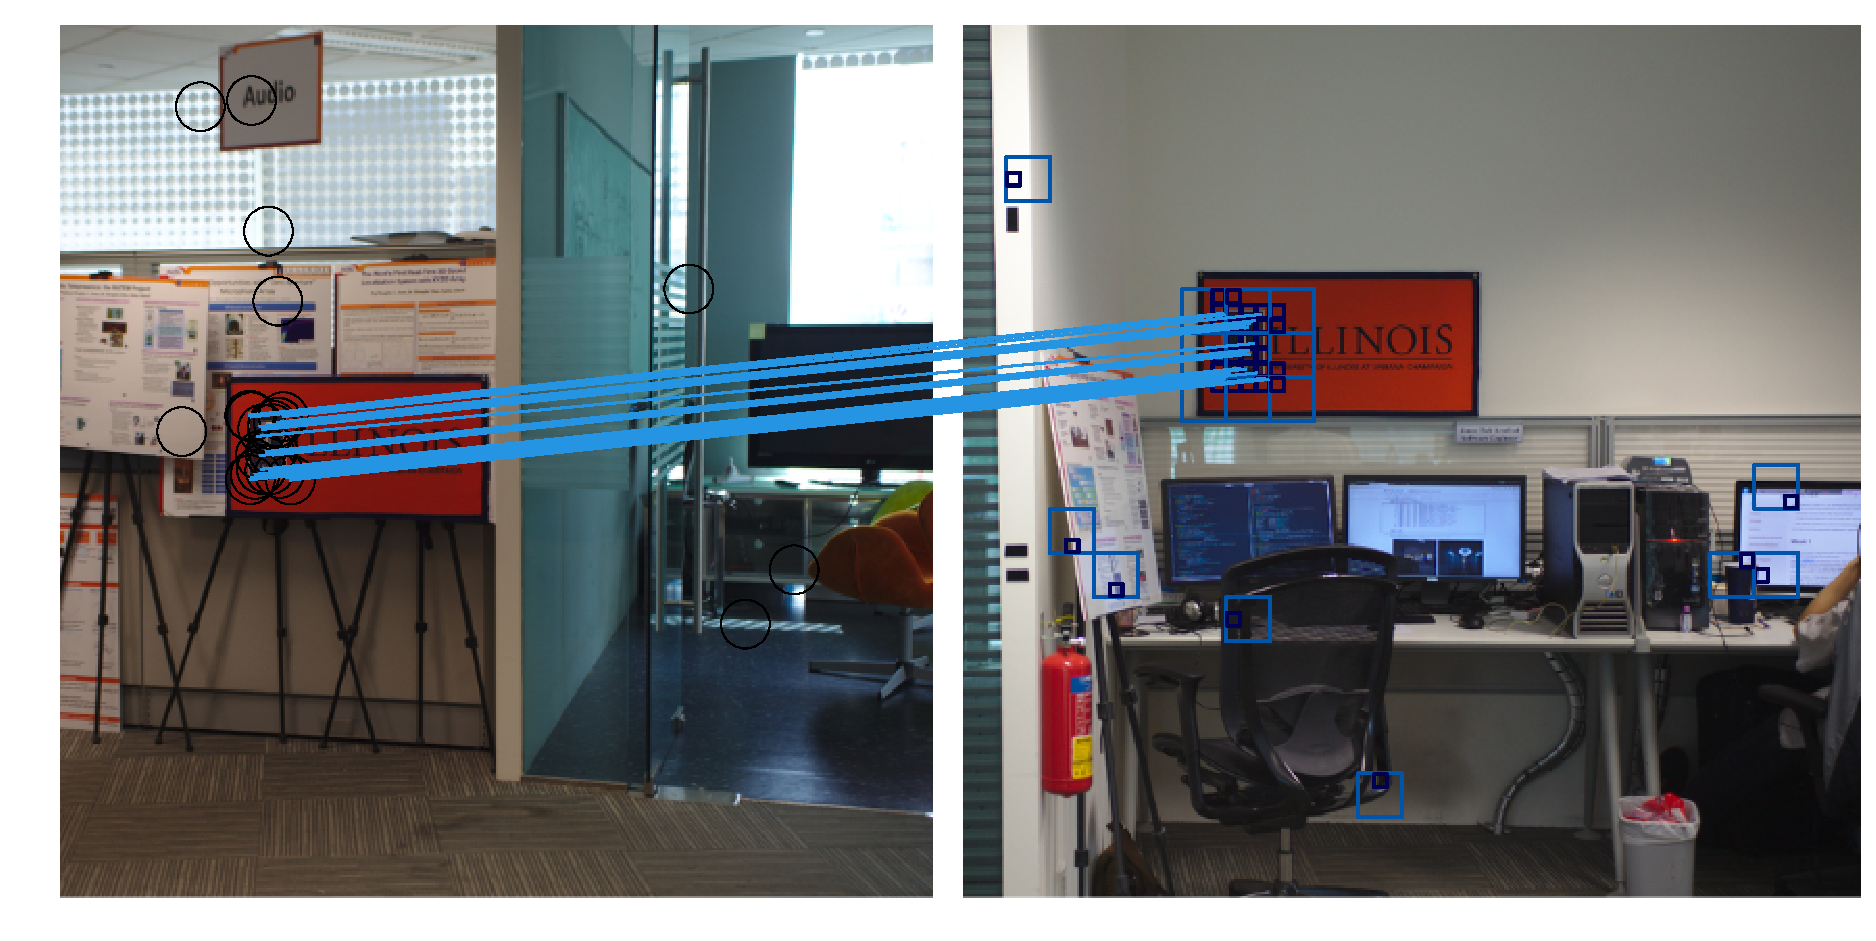
\includegraphics[width=1\columnwidth]{images/Illinois-fastmatch}
    \end{subfigure}%
    ~%\vspace{1.5 mm}
    \begin{subfigure}[t]{0.5\columnwidth}
        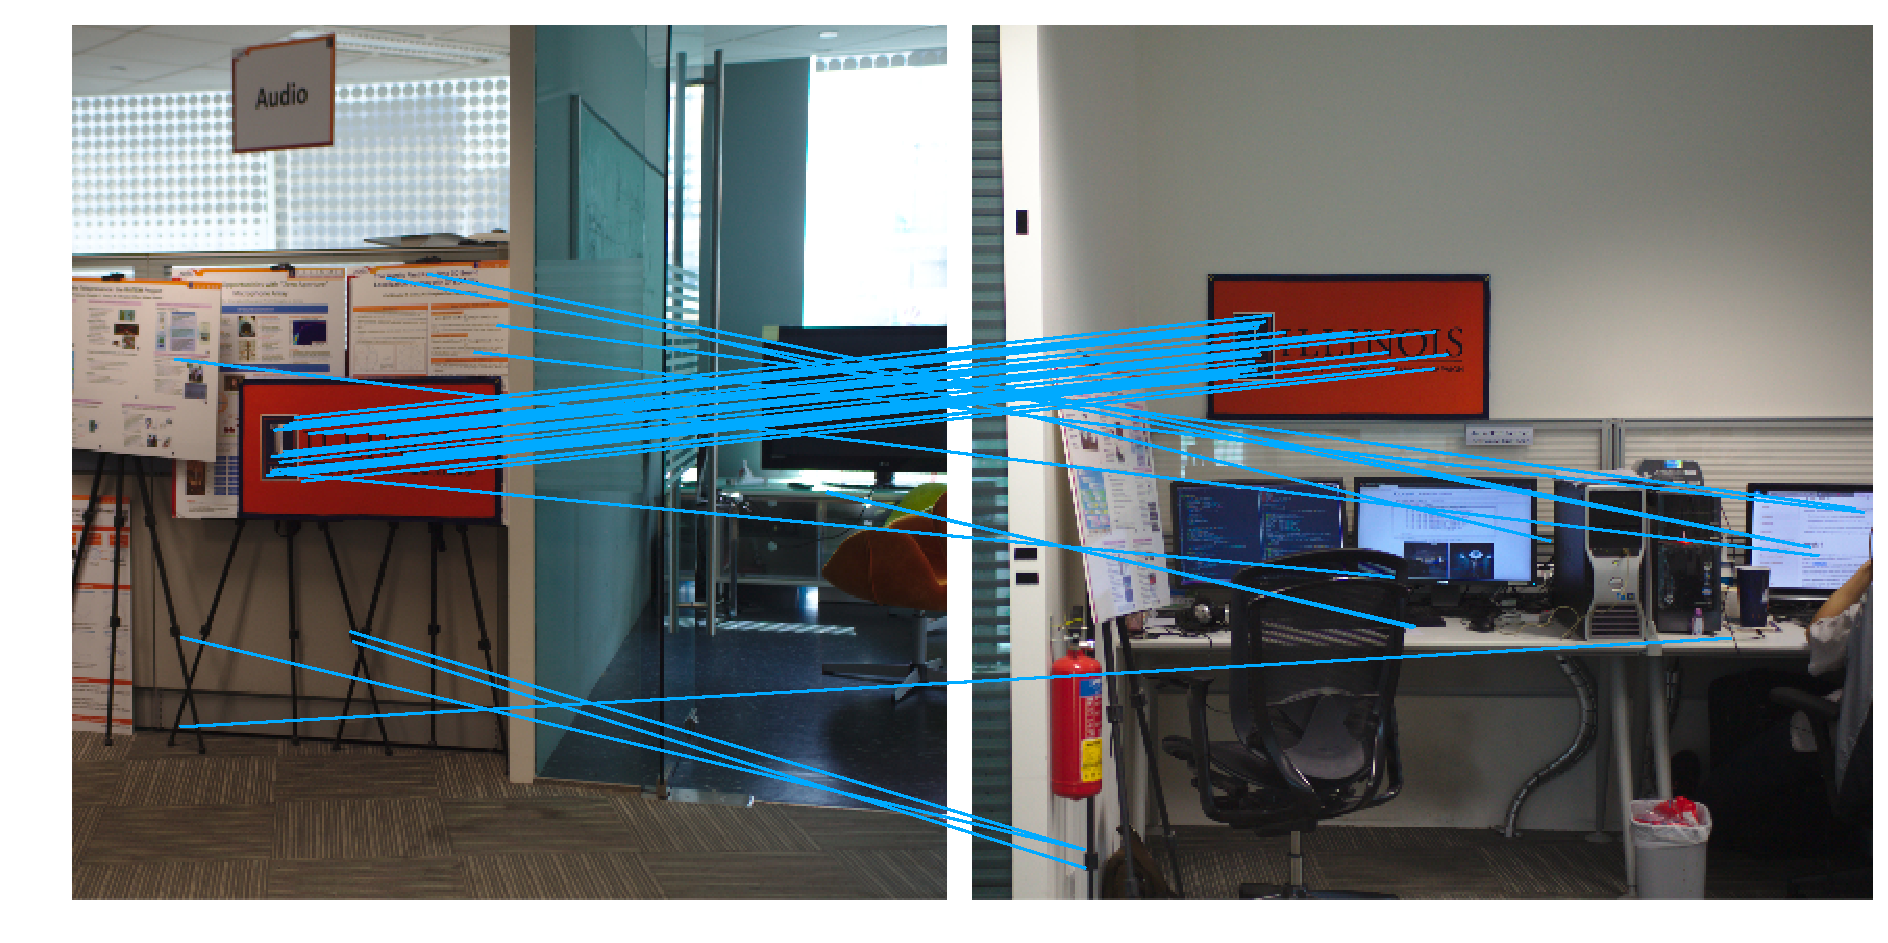
\includegraphics[width=1\columnwidth]{images/Illinois-ratiomatch}
    \end{subfigure}%
    \caption{The 50 best matches by the proposed \emph{Fast-Match} algorithm (left) and the \emph{Ratio-Match} algorithm \cite{lowe2004sift} (right). The lines between the image pairs denote a match as proposed by the algorithm. For \emph{Fast-Match} the zones of the right image where local features were computed has been marked with a blue square.}
    \label{fig:match_example}
\end{figure}

\section{Matching Fast and Slow}
\label{algorithm}
%
In this section we will introduce the fundamentals of \emph{Fast-Match} and motivate the design choices as we go. The algorithm consists of 3 components; finding seeds, finding matches, and exploring for other places where matches might be.

\subsection{Considerations}
\label{considerations}
%
If we set out to design a truly fast matching algorithm, we cannot rely just on optimizing the matching step once the descriptors from both images have been found and computed. Finding and computing descriptors can easily account for 80\% of the time spent matching for bigger images (cf.\ Figure~\ref{fig:timings}). For this reason \emph{Fast-Match} is designed to only compute features for the part of the image we hope to match. 

The \emph{Fast-Match} algorithm is demonstrated in Algorithm~\ref{alg-fast}. Given a \emph{query image} and a \emph{target image} that we intend to match and a confidence threshold $\tau$, we obtain a set of seed matches from the two images. For each seed match we look at the matched position in the \emph{query} and \emph{target images} and find a set of matches. We save these matches and their confidence scores; for those that pass the confidence threshold $\tau$, we obtain another set of seed matches. In this way we iterate until we have no more seed matches and return the matches and their confidence scores. In an intuitive sense $\tau$ serves as a parameter directing the thoroughness of the algorithm, i.e. how much time we spend matching, while the final precision and recall can be adjusted by thresholding the matches on their confidence scores at the end.

We a \emph{general} and a \emph{retrieval} variation of the algorithm. The latter assumes that we know one of the images that we intend to match ahead of time and can do some off-line computations. For the \emph{general} variation we make those computations on the fly instead and do not assume anything to be pre-computed. 

\begin{algorithm}[htb]
\caption{Fast-Match}
\label{alg-fast}
\begin{algorithmic}
    \Require $I_{query}, I_{target}$ : images, maxiter $\in \mathbb{N}$, $\tau \in [0,1]$
    \State $M_{seed} ~\gets$ seed\_matches$(I_{query}, I_{target})$
    \State $M_{final} \gets \varnothing$
    \State $C_{final}~ \gets \varnothing$
    \State $M_{seen} ~\gets \varnothing$
    \While{$M_{seed} \ne \varnothing \wedge i < $maxiter$}$
        \State $M_{round}~ \gets$ get\_matches$(M_{seed})$
        \State $C_{round}~\,\gets$ get\_confidence$(M_{round})$
        \State $M_{seed}~~~ \gets$ get\_seeds$(M_{round} \setminus M_{seen}, C_{round}, \tau)$
        \State $M_{seen}~~\,\gets M_{seen} \cup M_{seed}$
        \State $M_{final}~\,\gets M_{final} \cup M_{round}$
        \State $C_{final}~~\,\gets C_{final} \cup C_{round}$
    \EndWhile \\
    \Return $M_{final}, C_{final}$
\end{algorithmic}
\end{algorithm}

\subsection{Initiating Seeds}
\label{seeds}
%
Depending on the scenario, several strategies can be used to obtain a set of initial seed matches. For the case of matching a pair of two images we can get a rough group of seed matches by matching the thumbnails of the two images with for example \emph{Ratio-Match}. However if we were matching images in a series, such as frames from a movie we could instead make use of a subset of the matches from the last frame to seed \emph{Fast-Match} on the next. In practice we have found it efficient to resize both images to thumbnails of $300\times 300$ pixels and use ratio match to obtain a set of matches and ratios that we then threshold with the confidence threshold $\tau$ to obtain the initial seed matches.

\subsection{Collecting Matches and Computing Confidence}
\label{collection}
%
If a seed match yields a connection between two points $p_q$ in the \emph{query image} and $p_t$ in the \emph{target image}, then we are interested in collecting all matches between the regions $R_q$ and $R_t$ centered around $p_q$ and $p_t$ respectively. From each region we can extract a set of feature points between which we try to find a set of matches $M_{qt} $ and a set of confidence scores $C_{qt}$.

Lowe and others have shown that the distance between two SIFT descriptors is much less indicative of a true correspondence than the ratio between the best and second best match \cite{lowe2004sift,mikolajczyk2005performance,moreels2007evaluation,rabin2009statistical}. This ratio is more formally defined as follows: If we let $f_q$ be a feature in the \emph{query image} and $f_t, f_b$ be the two nearest neighbours of $f_q$ in the \emph{target image} then the ratio $r$ is defined as follows:
\begin{align*}
    r &= %\text{r}(f_{q}, (f_t, f_b)) \\
        &= \frac{d(f_{q}, f_{t})}{d(f_{q}, f_{b})}.
\end{align*}
Here $d(f_i,f_j)$ is the distance between the features $f_i$ and $f_j$. For SIFT this is the Euclidean distance. The distance between two feature points is greater when the feature points resemble each other less. For this reason we have higher confidence in a match with a low $r$-value. Using $r$ as a measure of match confidence presumes that we expect each feature in the \emph{target image} to have at most one true correspondence in the \emph{target image}. Intuitively if we try to find a match for a feature $f_i$ in an image that does not have any true correspondences, then we would expect the two closest neighbours to be roughly equally well matched with $f_i$. For this reason we attribute high confidence to matches where the closest neighbour is dramatically closer to $f_i$ than the second closest neighbour and discard the rest.

We are faced with a problem when applying this technique to obtain the set of confidence scores $C_{qt}$, since for any match in $M_{qt}$ we only know the nearest neighbours amongst the features of $R_q$ and $R_t$. To get around this problem we either assume to know one of the images beforehand (the \emph{retrieval} variation) or -- in case we cannot make that assumption -- we compute the features of one of the images (the \emph{general} variation). For a given match between features $f_q$ and $f_t$ we can now find the second closest neighbour neighbour $f_b$ and calculate the confidence as $r = d(f_q, f_t)/d(f_q,f_b)$.

In the retrieval scenario where we know an image beforehand, we can further optimize this step. If we assume the \emph{target image} is known in advance we can approximate the ratio by letting $\hat r = d(f_t, f_q)/d(f_t,f_b)$. Here the feature $f_b$ is also part of the target image, which means we can pre-calculate $d(f_t, f_b)$ for all features in the cached \emph{target image} before we start matching. When these distances are tied to their corresponding feature in the target image, it becomes trivial to calculate $\hat r$.

\begin{figure}[t]
\centering
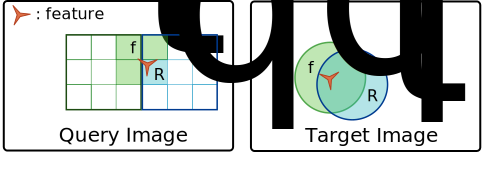
\includegraphics[width=0.75\columnwidth]{images/exploration}
\caption{Exploration of features based on match. The areas shaded blue are the areas that were searched to obtain the match. The areas shaded green are candidate areas for obtaining more matches.}
\label{fig:exploration}
\end{figure}

\subsection{Exploring for Matches}
\label{exploring}
%
In each iteration we compute a new set of seed matches, i.e.\ positions that might yield more matches in the image. For each region $R_i$ evaluated during the collection step we now have a set of matches $M_i$ and a set of confidence levels $C_i$ that we can use to predict whether the neighbourhood of $R_i$ is worth exploring.

There are many possible heuristics for predicting possible regions including local and global epipolar assumptions and partial graph isomorphisms. However, for the sake of simplicity and speed we have chosen a straightforward approach based on weak angular assumptions, as illustrated in Figure~\ref{fig:exploration}. Assuming that the \emph{target image} has been cached either in advance or before the matching step, the blue shaded areas show $R_q$ and $R_t$ for a given seed match. In the \emph{target image} we collect all features in a given radius while we compute features in the rectangular $R_q$ in the \emph{query image}. For performance reasons we compute all features in the blue square but match only the features inside the shaded area. Next a match is found in the collection step between $f_q$ and $f_t$. Based on the position of $f_q$ in $R_q$ we select three areas with potential for more matches. The center of each is matched with the center position $f_t$ to produce three seed matches for the next iteration. In Figure~\ref{fig:match_example} we illustrate this process in the \emph{Fast-Match} image pair. The \emph{query image} to the right in the figure has a small blue square for each region that has been used while matching the two images.

In practice it is necessary that these squares overlap in order to detect features lying close to the edges. This incurs a bit of overhead which is minimized by only collecting features for groups of 9 squares. In order to avoid computing the same matches or features twice, quite a bit of care has to be expended making sure that results are properly cached. A matrix containing `bins' of features can conveniently be used to store features from different image regions. Similarly a hash-set is suitable for keeping track of which regions have already been matched and which matches have already been found.

\subsection{Computational Complexity}
\label{complexity}
%
The difference between the \emph{general} and \emph{retrieval} variation of \emph{Fast-Match} consists in whether we compute the features in the \emph{target image} (general) or if we presume the features are computed offline (retrieval). Computing the features is linear in the number of feature points, while finding $d(f_q, f_b)$ for all $n$ features in the \emph{target image} can be done in $O(n\log n)$ using metric trees. 

Once the features and their distances have been computed, the algorithm iteratively finds new seed matches based on previous sets of seed matches. For each seed match we collect new matches, calculate confidence scores, and obtain new seed matches. Each of these steps varies only with the local region size which is constant. As a consequence the running time is linear in the amount of possible seed matches.

We will show that the number of possible seed matches is on average linear in the number of image features, and we also provide an upper bound for the probability that it is not. We assume that outside of true correspondences, features have better or at least equally good matches in terms of confidence in the image they come from. More rigorously put: For any feature in the target image $f_t$ let $f_1, f_2, \ldots$ be the best, second best, etc matching feature from either image which is not a true correspondence. Let $A_{ti}$ be the event that $f_i$ is found in the \emph{query image}, then $\mathbb{P}(A_{ti}) \leq 0.5$ and $A_{ti}$ is independent from $A_{tj}$ when $i \ne j$.

For a given feature in the \emph{target image} $f_t$, its nearest neighbour in the \emph{target image} $f_b$, and the set of features in the \emph{query image} $F_{query}$, we can define the stochastic variable $X_t$ as follows:
\begin{align}
    X_t = \left| \{ \, f_q \, \middle| \, f_q \in F_{query},\, d(f_q, f_t) < d(f_q, f_b) \} \right|
\end{align}
That is, $X_t$ is the number of features in the query image closer to $f_q$ than $f_b$. For each feature $f_t$, $X_t$ is an i.i.d.~stochastic variable. 

In the worst case, each feature in the \emph{target image} has a true correspondence in the \emph{query image} and $\mathbb{P}(A_{ti} = 0.5)$, in which case we find can find $\mathbb{P}(X_t = n) = \mathbb{P}(A_{ti})^n = 0.5^n$, as well as the expected value $\mathbb{E}(X_t) = \sum_{i=1}^\infty i0.5^i = 2$, and the variance $Var(X_t) = \sum_{i=1}^\infty 0.5^i(i - 2)^2 = 6$.

For $\tau = 1$ we accept a seed match when $d(f_t, f_q) \leq d(f_t, f_b)$. That means that for any feature in the \emph{query image}, we accept at most $X_t$ matches. To find the total amount of seed matches given $n$, we let $S_n = X_1 + \ldots + X_n$, in which case $\mathbb{E}(S_n) = 2n$. This proves that the expected amount of seed matches is linear in the number of target features. 

For the above case it is theoretically possible that for every one of the $n$ features we end up considering $kn$ seed matches for some constant $k$, i.e.\ a quadratic behaviour. Using Chebyshev's inequality we can provide an upper bound on the probability of this event:
\begin{align}
    \label{bound}
    \mathbb{P}\left(\left| \frac{S_n}{n} - \mathbb{E}(X_t) \right| \ge kn\right) &\le \frac{Var\left(\frac{S_n}{n}\right)}{k^2n^2} = \frac{6}{k^2n^3}
\end{align}

It is clear that for any constant $k$ we can pick a number of features $n$ which render the likelihood of a quadratic behaviour infinitesimal. In essence the larger $n$ becomes, the less likely \emph{Fast-Match} is to exhibit super linear behaviour.

The noteworthy part of this result is that for the \emph{retrieval} variation we can match two images in $O(n)$. Since there are no large constants involved this makes it possible to rapidly match very large images. In particular \emph{Fast-Match} is suited for cases where we are looking to match several large \emph{query images} to one \emph{target image}. In this case we can compute the features and distances of the \emph{target image} and then match each \emph{query image} in linear time. In contrast the general variation still has a complexity of $O(n \log n)$ due to the necessity of calculating distances online.

\section{Experimental Setup}
\label{experiments}
%
We evaluate \emph{Fast-Match} over 3024 image pairs featuring various 3D objects at different angles to measure precision and recall, as well as two pairs of images with high pixel counts to measure performance in terms of speed. We compare the algorithm to the standard \emph{Ratio-Match} \cite{lowe2004sift} as well as the newer \emph{Mirror-Match} \cite{arnfred2013mirror}. These two algorithms were selected because they are magnitudes faster than the fastest geometric algorithms while at the same time providing robust matches.

\subsection{Evaluation of Fast-Match on 3D Objects}
\label{3dobjects}
%
The 3D Objects dataset by Moreels and Perona \cite{moreels2007evaluation} allows us to experimentally compare matching algorithms over a large range of object and surface types rotated on a turnstile and photographed from every angle in increments of 5 degrees. 15 objects from the dataset are shown in Figure~\ref{fig:3d_objects}.  We use images of 84 different objects photographed under three different lighting conditions at 12 different angle intervals, conducting experiments with a total of 3024 image pairs. All photos a taken with a consumer camera in 3.1 megapixel resolution.

\begin{figure}[htb]
    \centering
    \begin{subfigure}[t]{0.15\columnwidth}
        \centering
        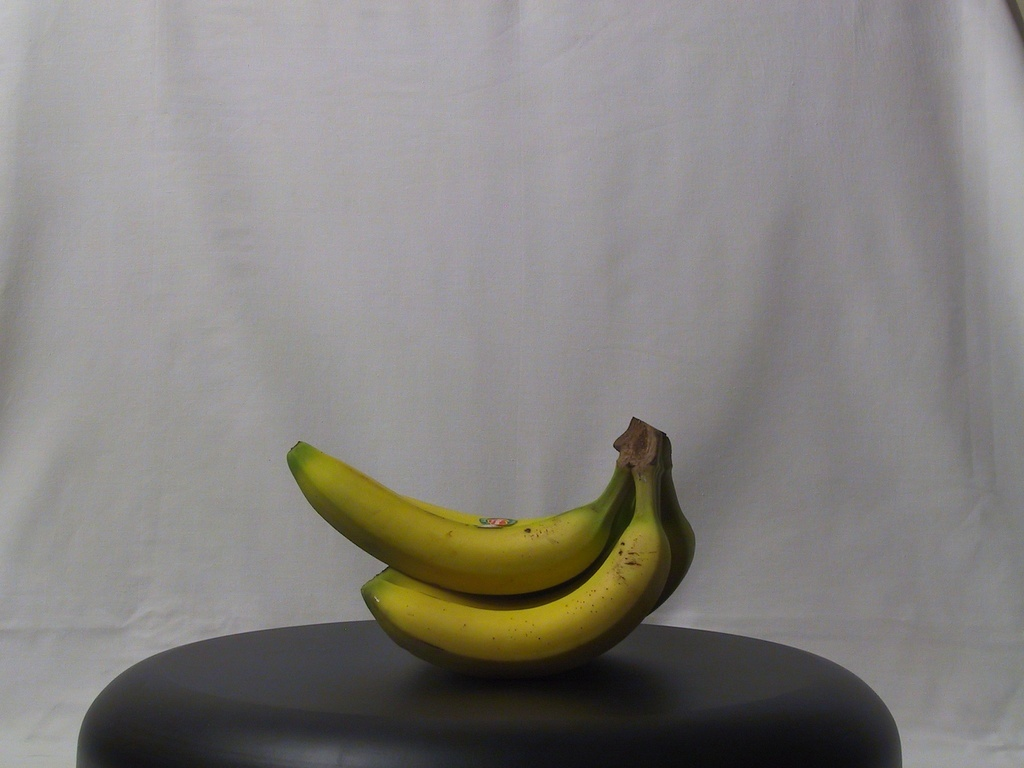
\includegraphics[width=1\columnwidth]{images/3d/1}
    \end{subfigure}%
    ~ %
    \begin{subfigure}[t]{0.15\columnwidth}
        \centering
        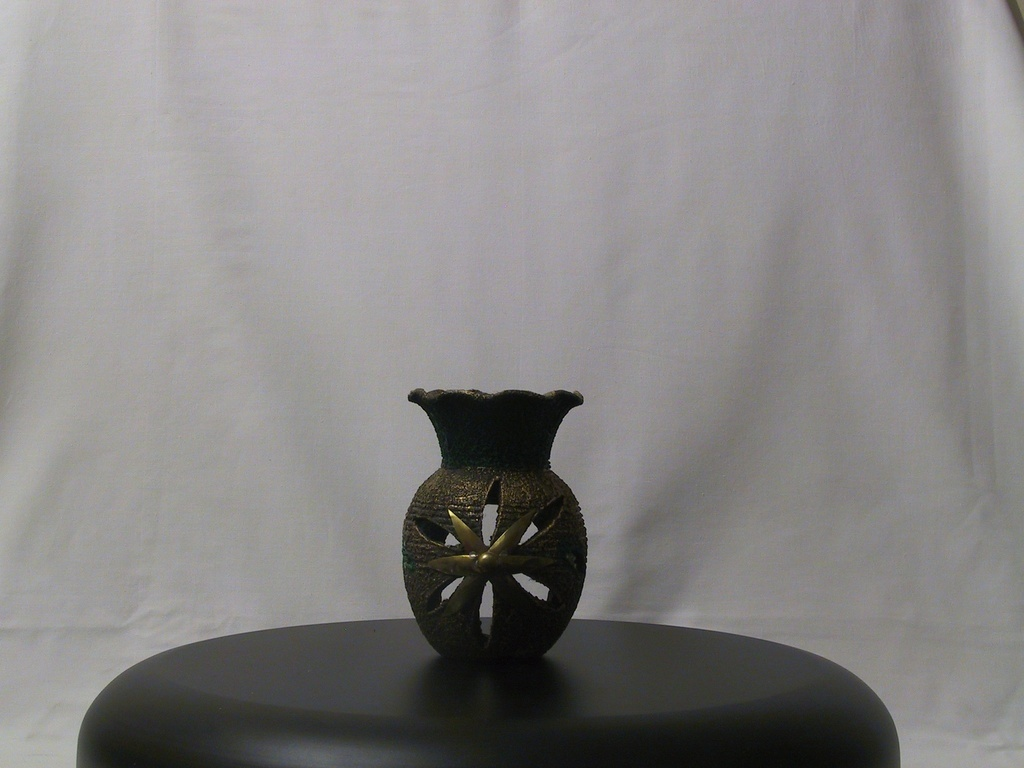
\includegraphics[width=1\columnwidth]{images/3d/2}
    \end{subfigure}%
    ~ %
    \begin{subfigure}[t]{0.15\columnwidth}
        \centering
        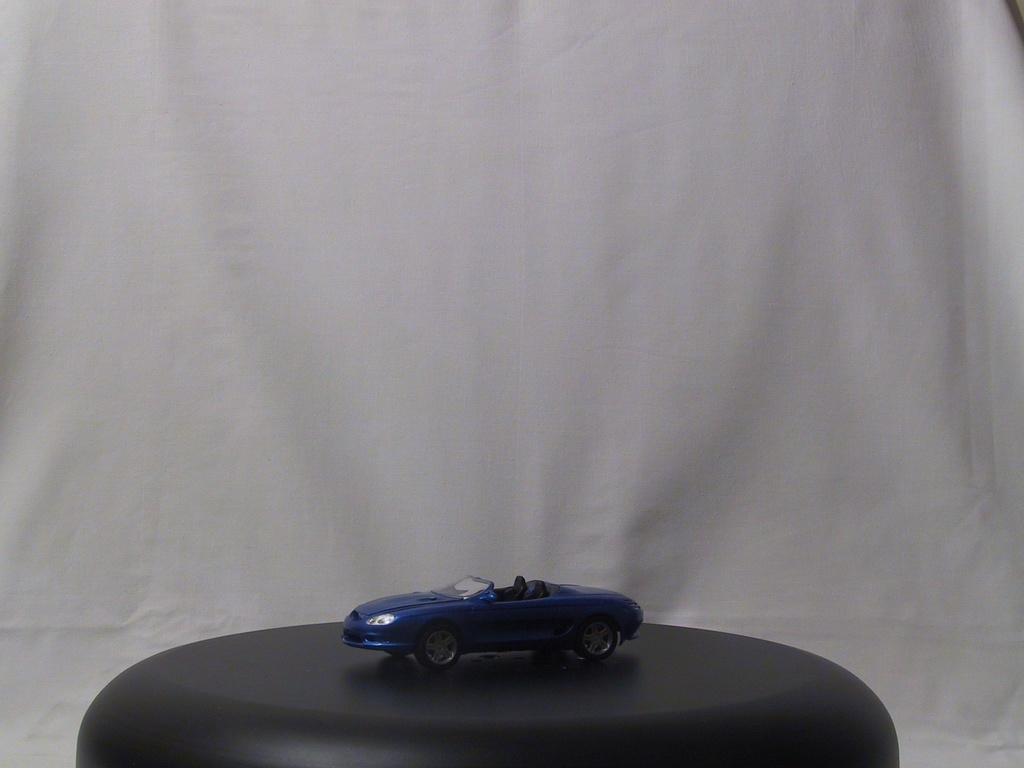
\includegraphics[width=1\columnwidth]{images/3d/3}
    \end{subfigure}%
    ~ %
    \begin{subfigure}[t]{0.15\columnwidth}
        \centering
        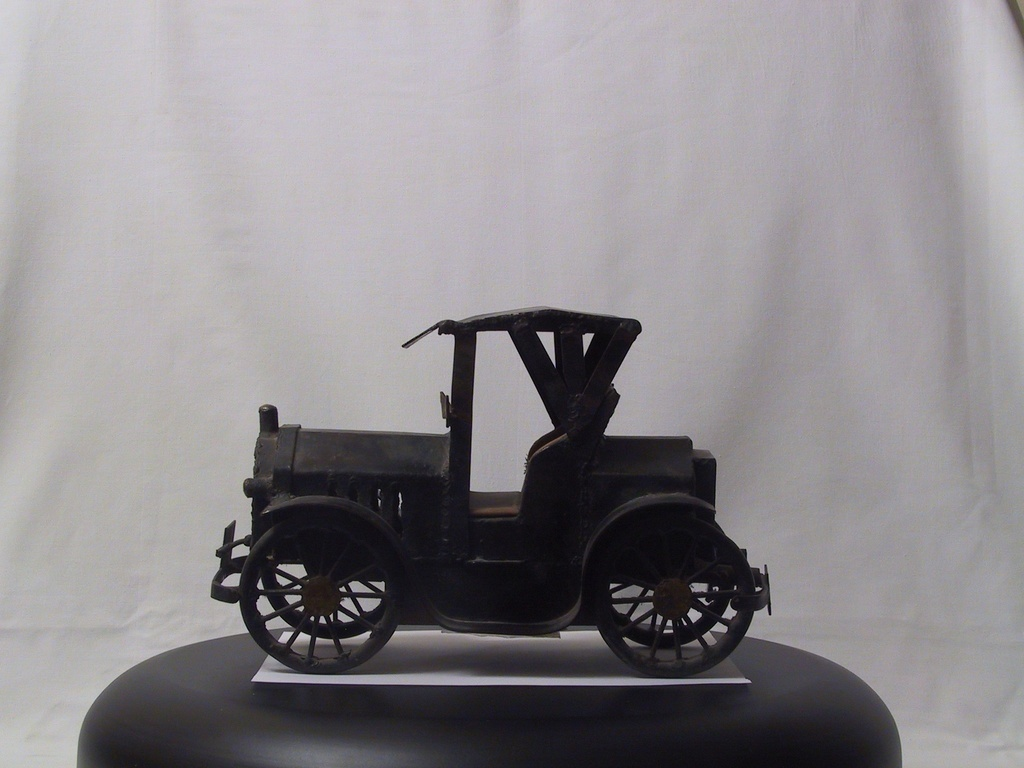
\includegraphics[width=1\columnwidth]{images/3d/4}
    \end{subfigure}%
    ~ %
    \begin{subfigure}[t]{0.15\columnwidth}
        \centering
        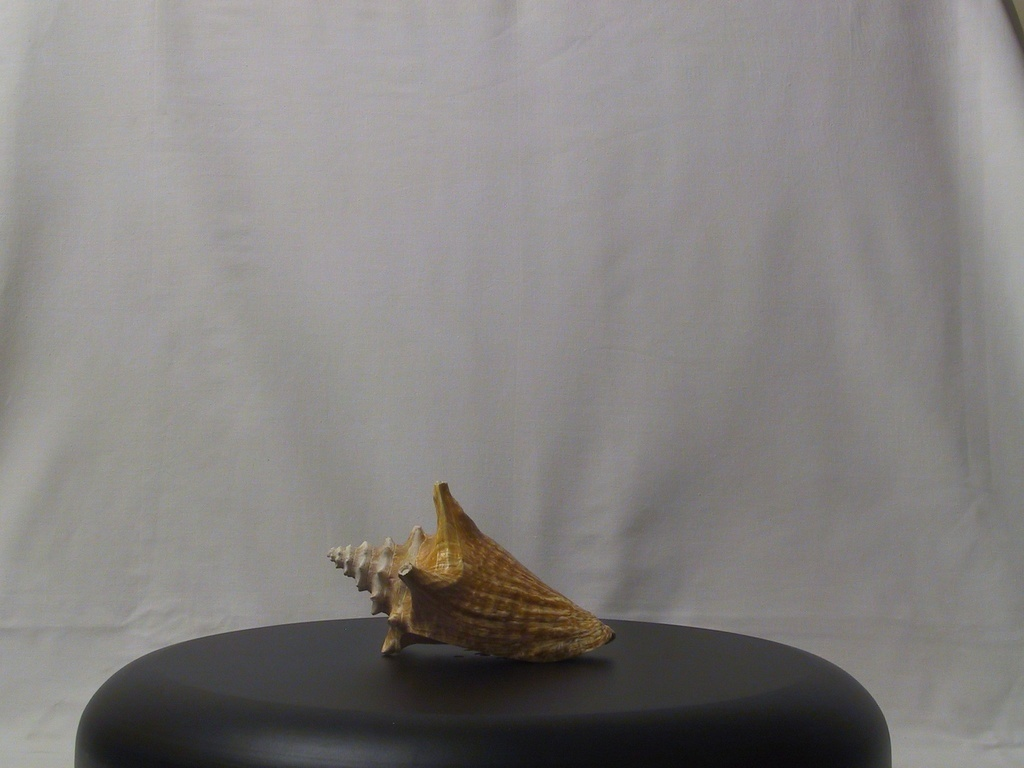
\includegraphics[width=1\columnwidth]{images/3d/5}
    \end{subfigure}%
    \vspace{1.5 mm}

    \begin{subfigure}[t]{0.15\columnwidth}
        \centering
        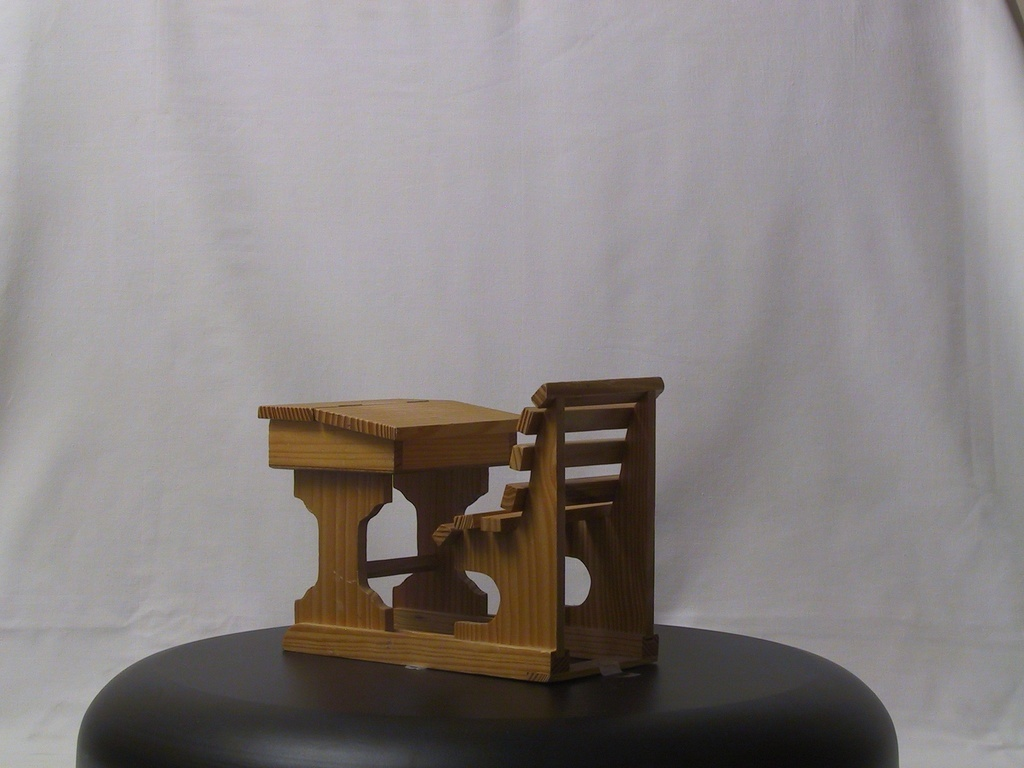
\includegraphics[width=1\columnwidth]{images/3d/6}
    \end{subfigure}%
    ~ %
    \begin{subfigure}[t]{0.15\columnwidth}
        \centering
        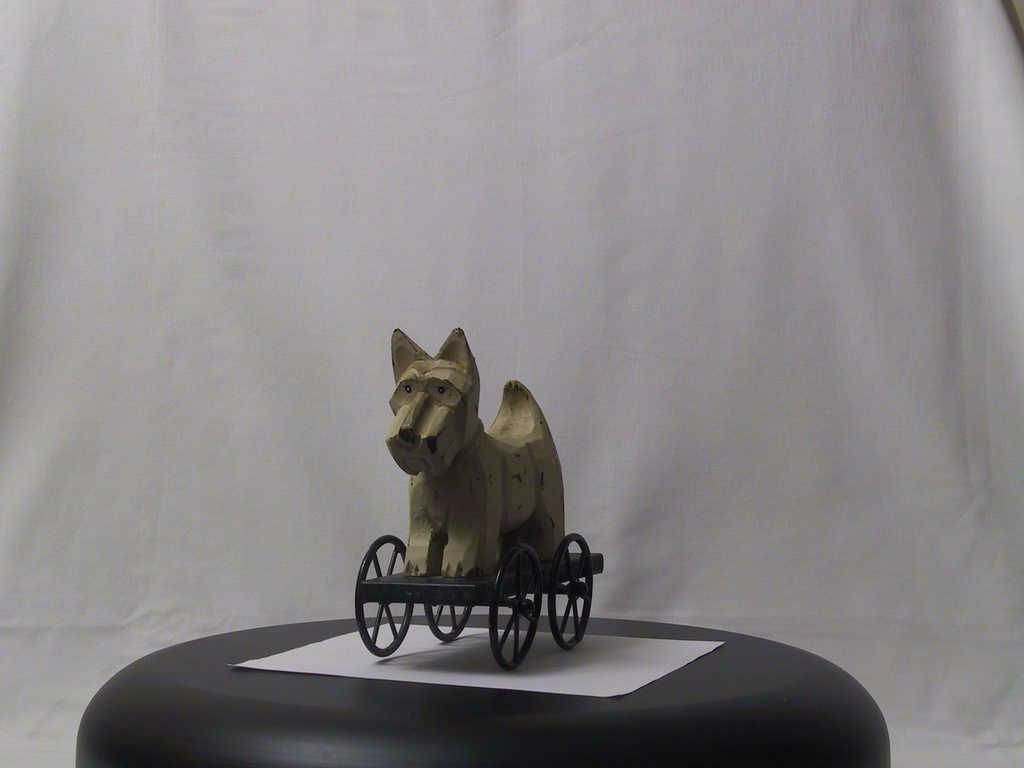
\includegraphics[width=1\columnwidth]{images/3d/7}
    \end{subfigure}%
    ~ %
    \begin{subfigure}[t]{0.15\columnwidth}
        \centering
        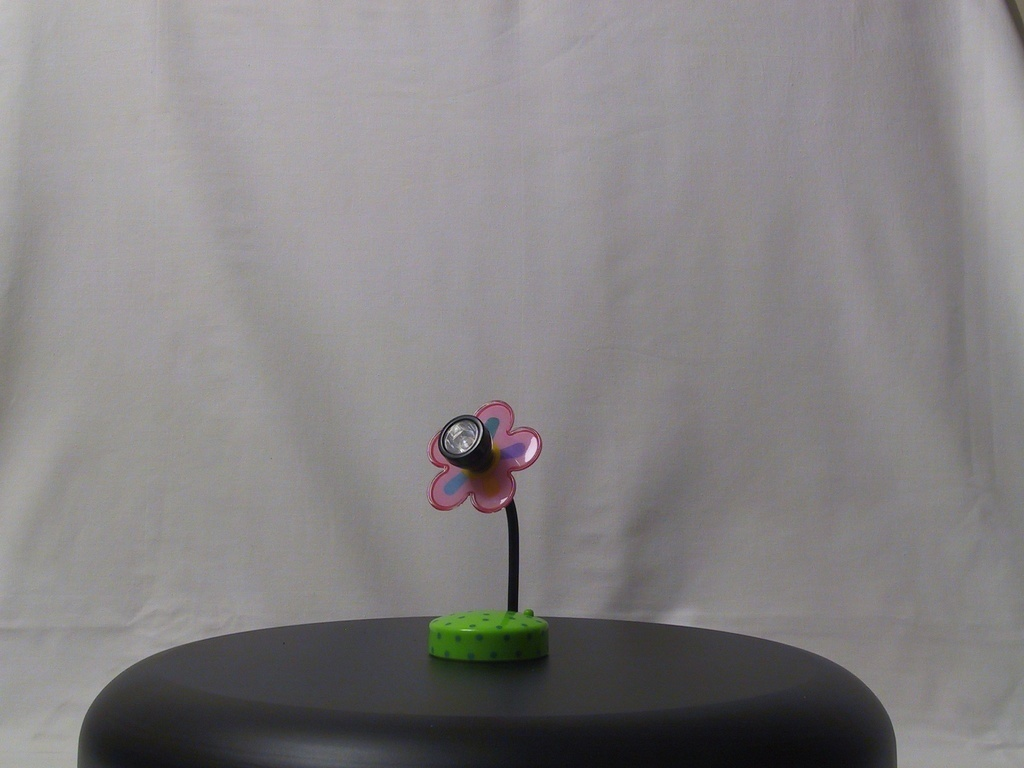
\includegraphics[width=1\columnwidth]{images/3d/8}
    \end{subfigure}%
    ~ %
    \begin{subfigure}[t]{0.15\columnwidth}
        \centering
        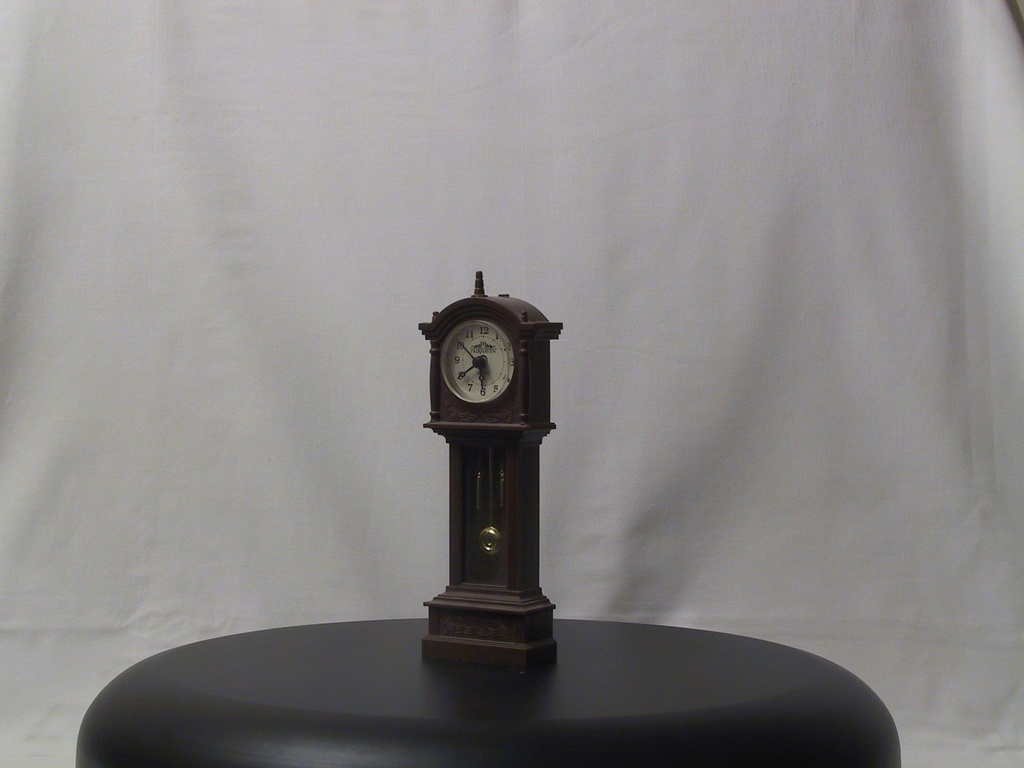
\includegraphics[width=1\columnwidth]{images/3d/9}
    \end{subfigure}%
    ~ %
    \begin{subfigure}[t]{0.15\columnwidth}
        \centering
        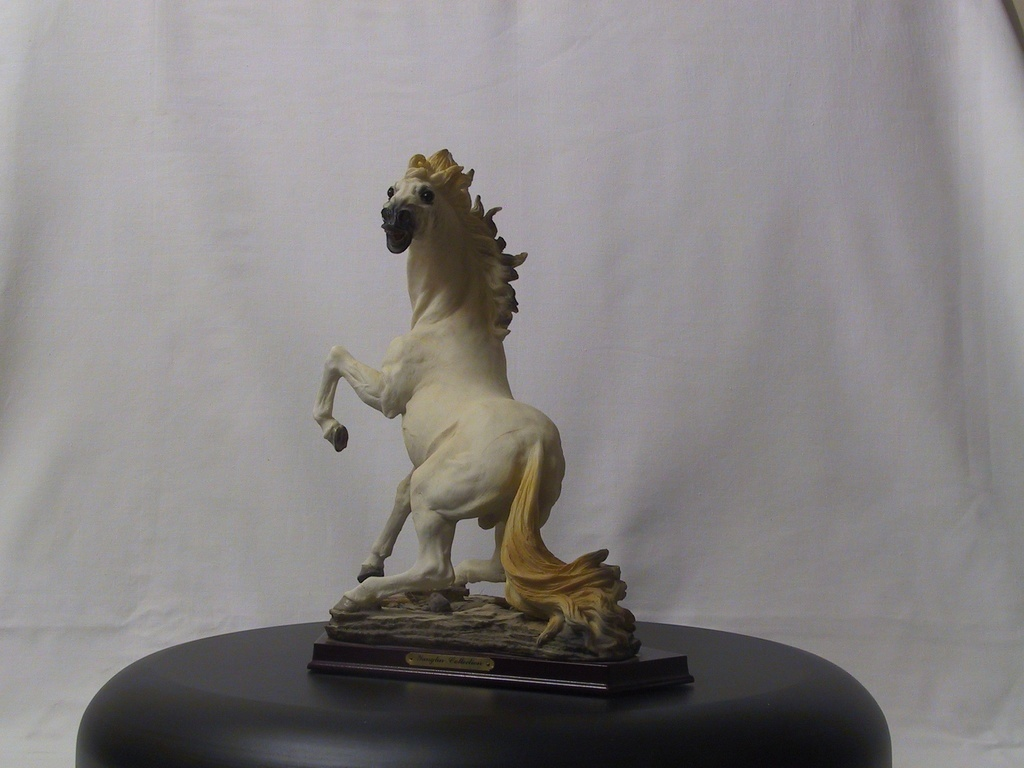
\includegraphics[width=1\columnwidth]{images/3d/10}
    \end{subfigure}%
    \vspace{1.5 mm}

    \begin{subfigure}[t]{0.15\columnwidth}
        \centering
        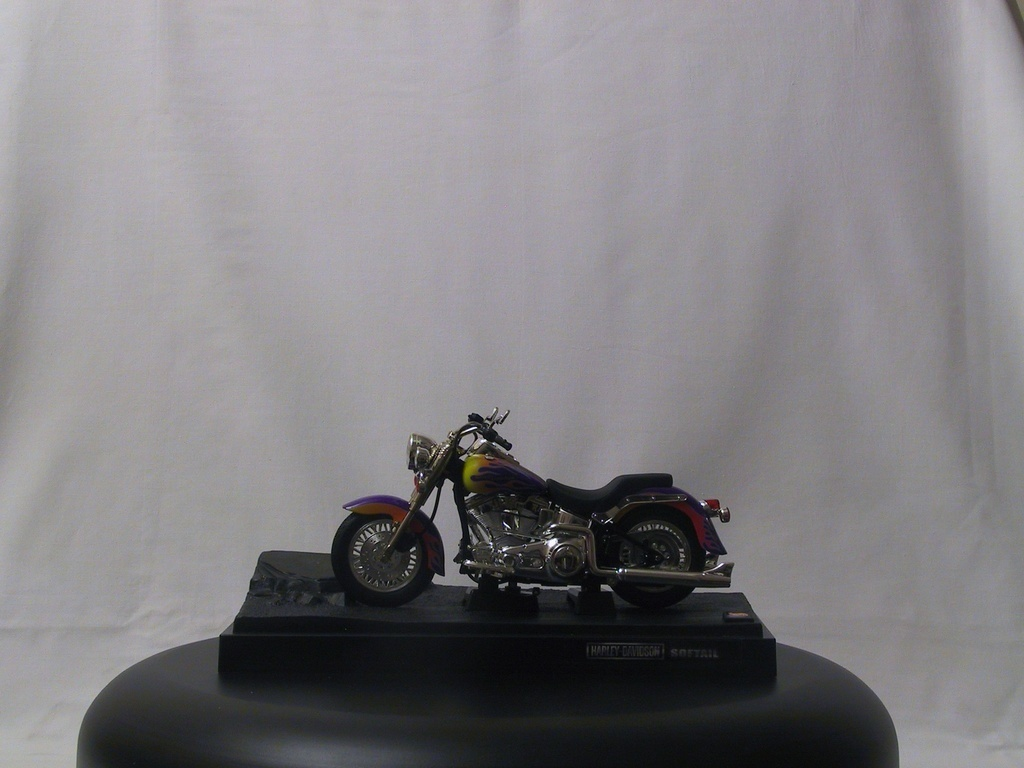
\includegraphics[width=1\columnwidth]{images/3d/11}
    \end{subfigure}%
    ~ %
    \begin{subfigure}[t]{0.15\columnwidth}
        \centering
        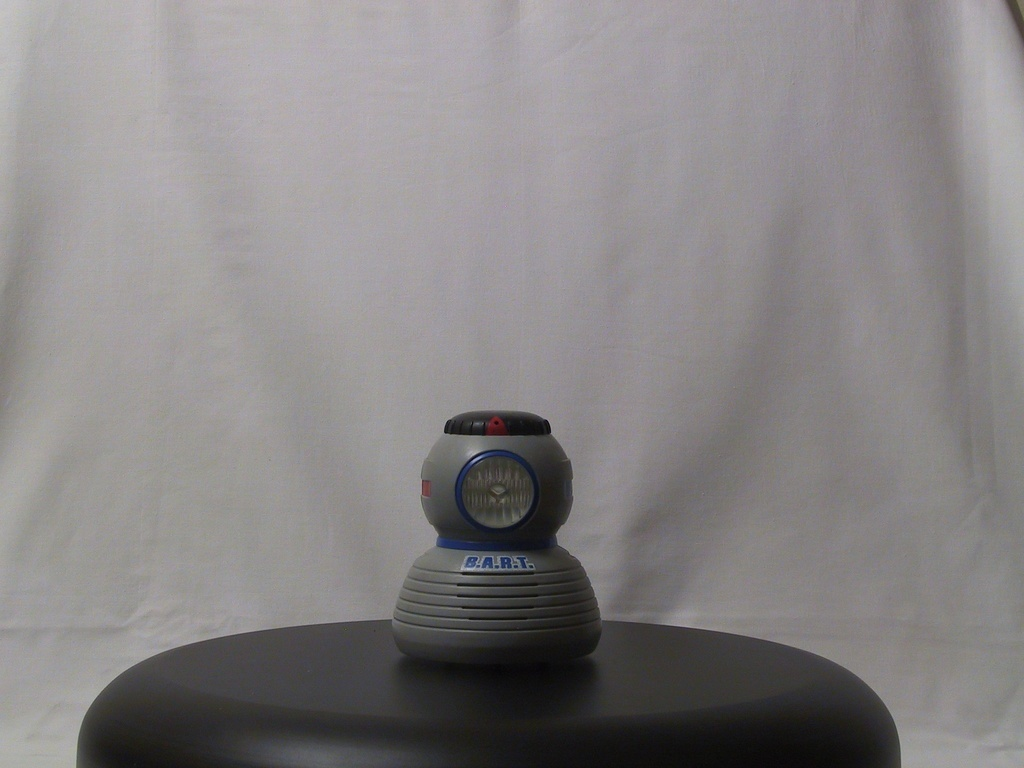
\includegraphics[width=1\columnwidth]{images/3d/12}
    \end{subfigure}%
    ~ %
    \begin{subfigure}[t]{0.15\columnwidth}
        \centering
        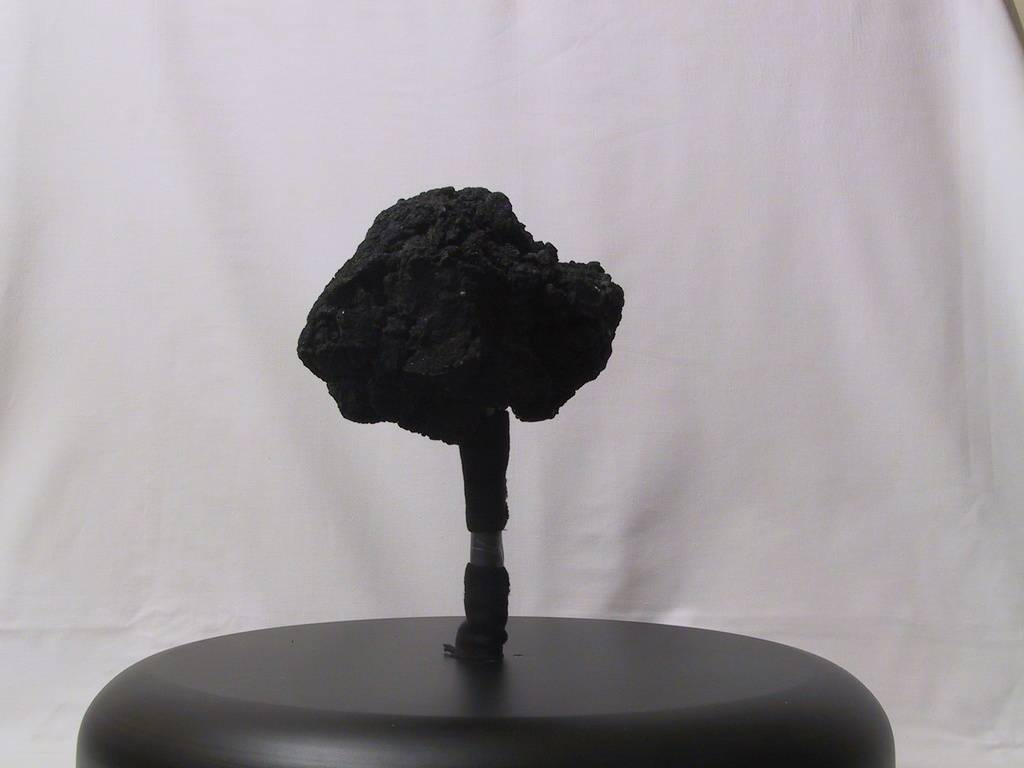
\includegraphics[width=1\columnwidth]{images/3d/13}
    \end{subfigure}%
    ~ %
    \begin{subfigure}[t]{0.15\columnwidth}
        \centering
        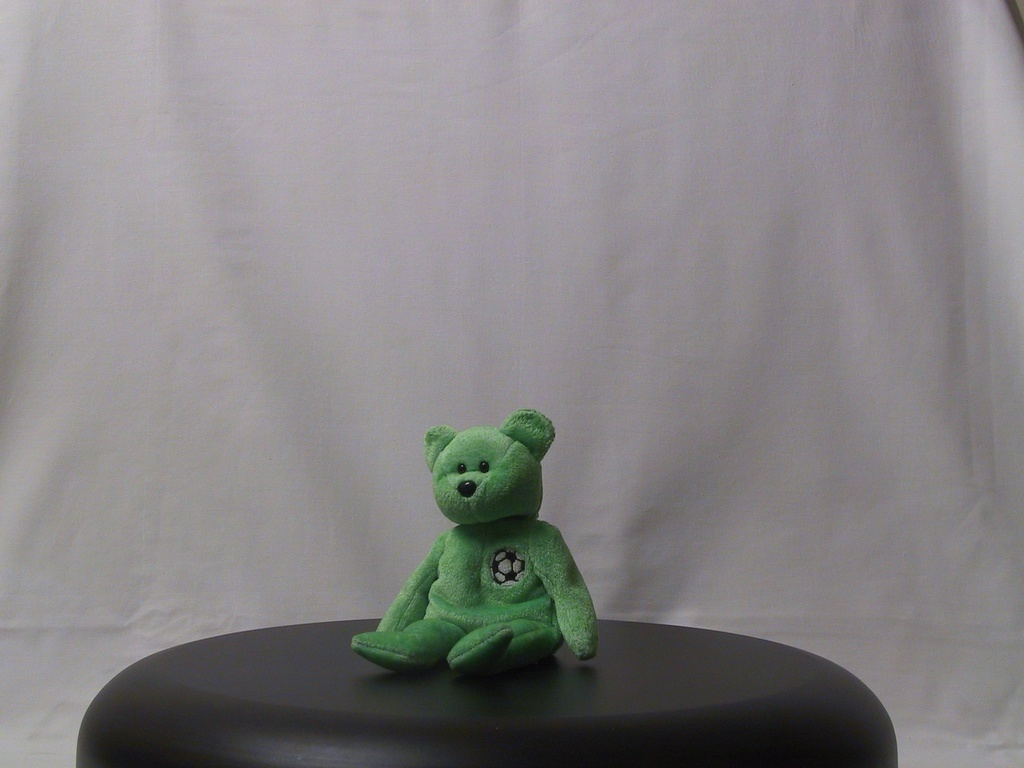
\includegraphics[width=1\columnwidth]{images/3d/14}
    \end{subfigure}%
    ~ %
    \begin{subfigure}[t]{0.15\columnwidth}
        \centering
        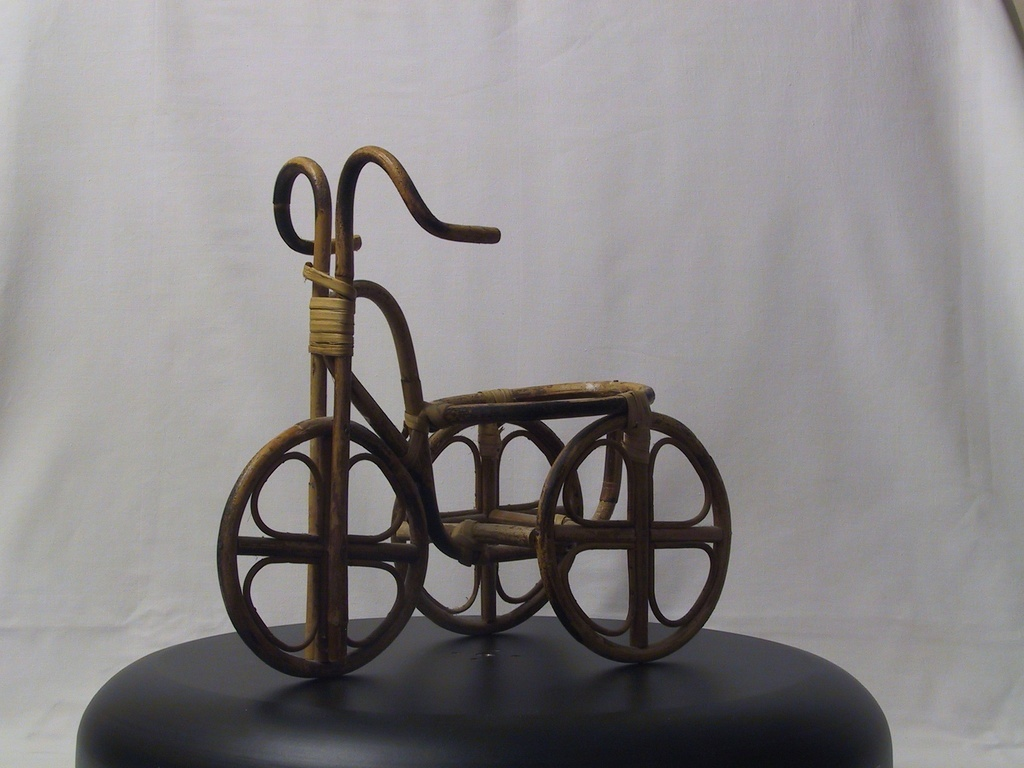
\includegraphics[width=1\columnwidth]{images/3d/15}
    \end{subfigure}%
    \vspace{1.5 mm}

    \caption{15 objects from the 3D Objects dataset by Moreels
    and Pietro \cite{moreels2007evaluation}.}
    \label{fig:3d_objects}
\end{figure}

To validate matches, Moreels and Perona propose a method using epipolar constraints \cite[p.266]{moreels2007evaluation}.  According to their experiments, these constraints are able to identify true correspondences with an error rate of $2\%$. We use their proposed method to generate the ground truth for the evaluation of our framework.

To compute the total number of possible true correspondences, we take each feature in a \emph{query image} and count how many of them have a feature in the \emph{target image} which would satisfy the epipolar constraints. When using this dataset, features with no correspondences were not included in the set of features for testing, so as to avoid matching non-moving background and foreground objects.

We evaluate all matching algorithms from our framework on the 3D Objects dataset by matching images at different angular intervals. For each object we pick the \emph{query} image as the image taken at 10 degrees rotation for calibration stability.  We then match this image with the same object turned an additional $\Delta$ degrees, $\Delta \in \{5, 10, \ldots, 60\}$.  For every angle interval we compare images taken under 3 different lighting conditions as provided by the dataset. We include all objects in the database for which photos at 5 degree angle intervals are available except for the ``Rooster'' and ``Sponge'' objects due to image irregularities.

\subsection{Configuration of \emph{Fast-Match}}
%
The central parameters of \emph{Fast-Match} are the confidence threshold $\tau$ for selecting seed matches and the final confidence threshold applied to the total set of matches. For the experiments on the 3D Objects we let $\tau = 0.9$ and created precision/recall plots by varying the confidence threshold over the final set of matches. 

To achieve a good balance between speed and robustness we let the region in which we extract features be a square with a side length of 90 pixels. On empirical tests we found that anything smaller would result in decreased performance while much bigger regions would decrease speed. The 90 pixel window is split in to nine smaller squares (see also Figure~\ref{fig:exploration}). When a seed match falls in any of these squares we match only the features within the smaller square. We let both the regions and the smaller squares overlap each other at all edges with 25 pixels in order to capture feature points lying close to an edge. For the image we have already cached we find all features within a radius of 50 pixels of the seed match.

\section{Results}
\label{results}
%
\begin{figure}[t]
\centering
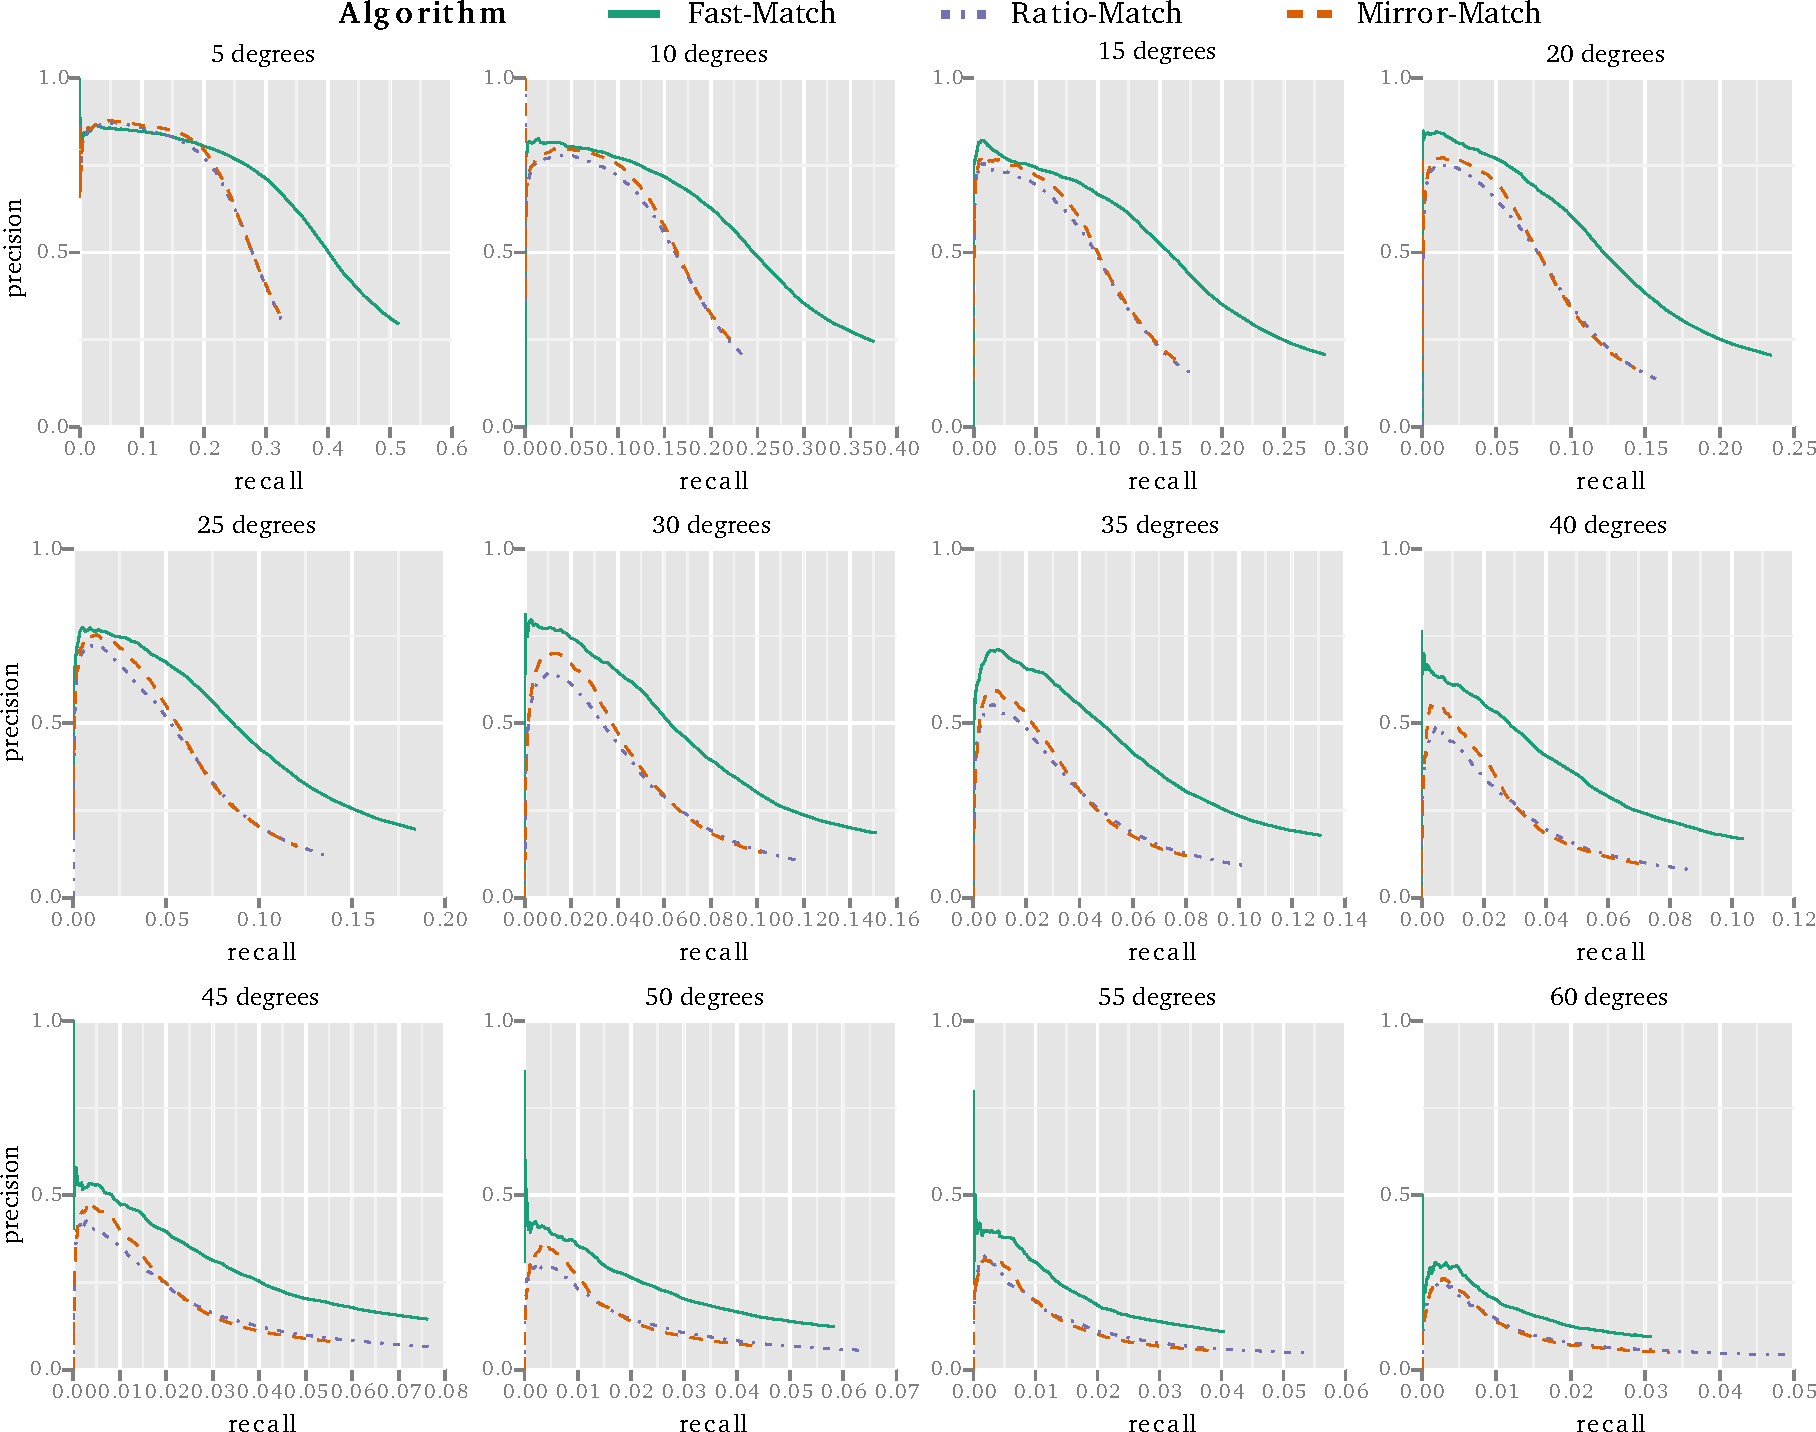
\includegraphics[width=1\columnwidth]{images/grid_match_all}
\caption{Results for the 3D Objects dataset. Each plot contains data accumulated from 84 objects photographed under 3 different lighting conditions.}
\label{fig:all_objects}
\end{figure}

Figure~\ref{fig:all_objects} shows the performance of the different matching methods in our proposed framework for $12$ increasingly bigger angle differences. The results are shown in a precision-recall plot to make it easy to compare performance in terms of precision at similar levels of recall.  For each plot we show the accumulated results on all 3D objects, weighted by the number of possible true correspondences for the individual objects. This ensures that each object contributes equally to the final result, despite some objects resulting in disproportionally more matches than others.

At low angular differences all algorithms show similar performance at low recall, however \emph{Fast-Match} is superior to \emph{Ratio-Match} and \emph{Mirror-Match} at higher recall, more than doubling the precision at similar recall levels. This picture remains the same at higher angular differences, but with a higher performance gap between \emph{Fast-Match} and the other algorithms at low recall while more than doubling precision at higher recalls. For image pairs with angular differences of more than 40$^{\circ}$ the performance of all algorithms declines, with \emph{Fast-Match} still coming out on top. 

The high recall rates of \emph{Fast-Match} are partially explained by the fact that we can allow our confidence thresholds to be more lenient when we already know that we are likely to find true correspondences in the regions that we are matching. However, lenient thresholds can easily impact the matching speed, so in practical situations we usually have to choose between matching fast and precisely, or more slowly with higher recall. 

\begin{figure}[tb]
    \centering
    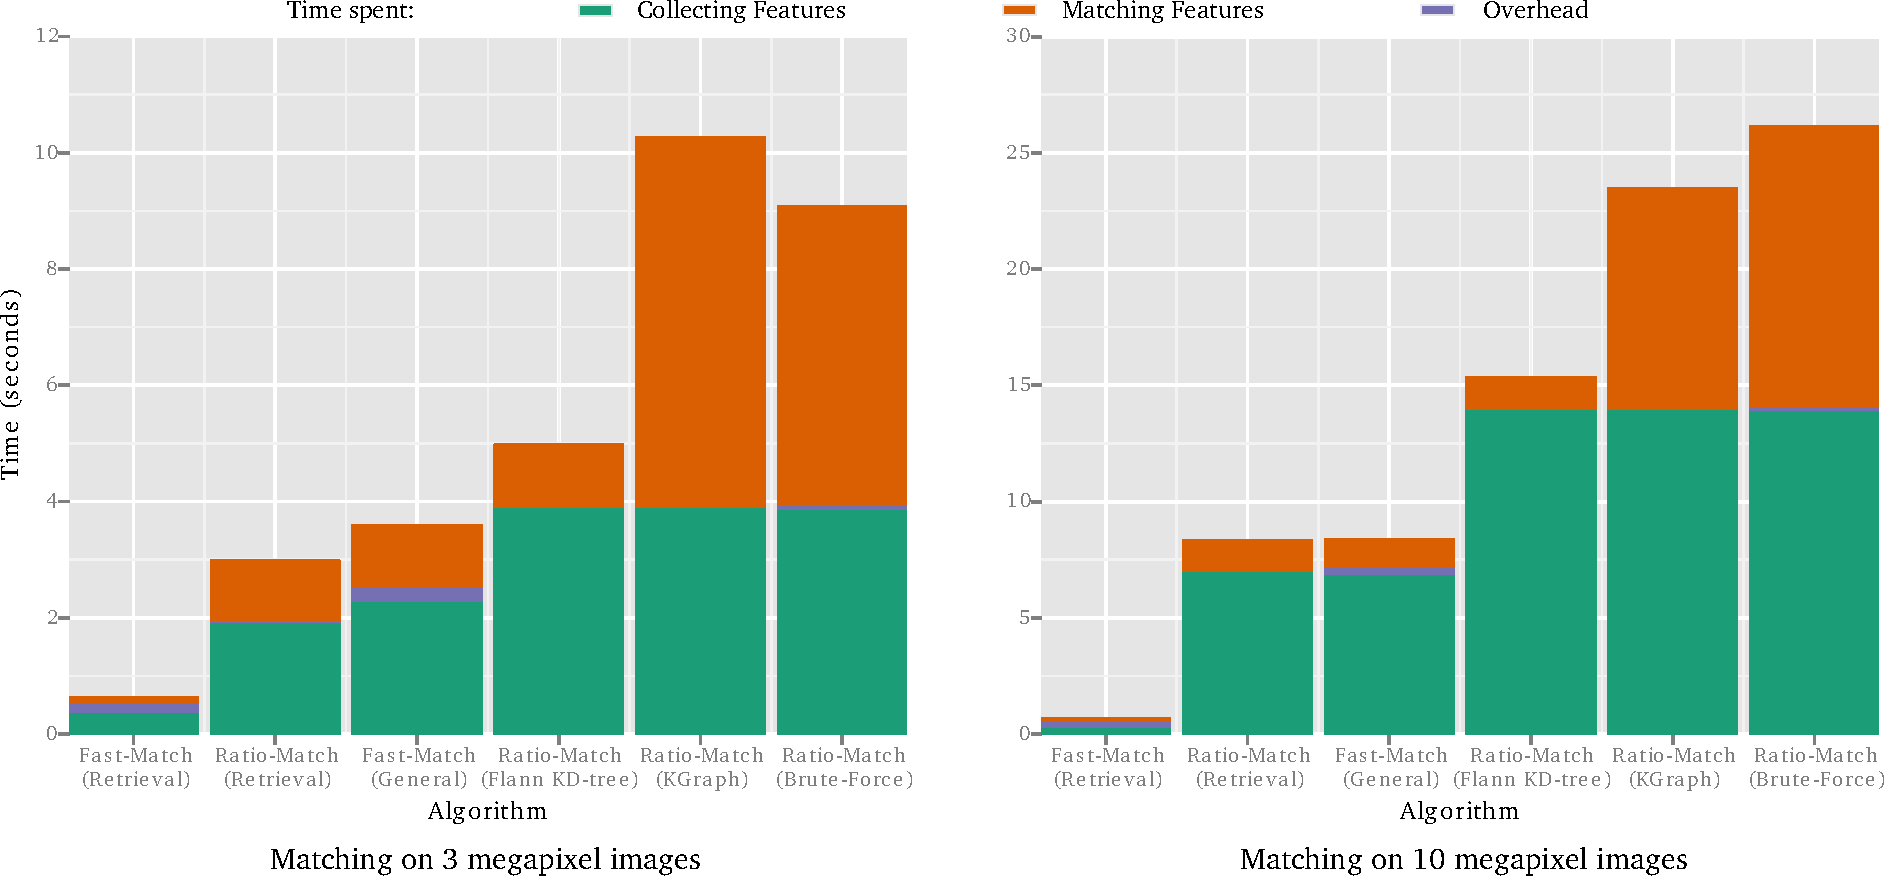
\includegraphics[width=1\columnwidth]{images/timings}
    \caption{The duration in seconds of different variations of \emph{Fast-Match} and \emph{Ratio-Match}. The top plot shows results for two 10~MPixel images two 3~Mpixel images is used for the comparison at the bottom. From the left, the first two results presume a precached image while the rest do not require knowing any inputs beforehand. The image pairs used be seen in Figure~\ref{fig:match_example}}
    \label{fig:timings}
\end{figure}

Figure~\ref{fig:timings} demonstrate the speed of \emph{Fast-Match} on image sizes as is typically produced by modern consumer cameras and camera phones. In Figure~\ref{fig:timings} we compare the speed of the two variations of \emph{Fast-Match} to different variations of \emph{Ratio-Match} on two image pairs, one with two images of 10 megapixel and another where the same image pair has been scaled to 3 megapixels. For the larger images we see the clearest difference in performance. The retrieval variant of \emph{Fast-Match} matches the image pairs in around one second while a retrieval variant of \emph{Ratio-Match} with precomputed features spends eight seconds on the same task. This result is roughly equal to the time the general variation of \emph{Fast-Match} spends matching the two images without any pre-computations. For the nearest neighbor search we note that for large images there are substantial speed gains to be had by choosing the right algorithm for finding nearest neighbors, with Muja et al.'s Flann matcher being vastly superior to brute force and KGraph. 

For the 3 megapixel picture the pattern repeats itself, although with smaller margins separating \emph{Fast-Match} and \emph{Ratio-Match}. When images are smaller, computations like obtaining the initial seed matches are comparatively more costly.

Figure~\ref{fig:match_example} shows the result from matching the pair of three megapixel images using \emph{Fast-Match} and \emph{Ratio-Match}. %An almost identical result can be obtained using the pair of 10 megapixel pictures instead. 
\emph{Fast-Match} ends up only matching the part of the images that are likely to have correspondences. This highlights both a strength and a weakness of \emph{Fast-Match}. It is this myopic matching approach that is responsible for \emph{Fast-Match}' speed and precision; on the other hand, \emph{Fast-Match} is not the best candidate for images that are almost identical, because its step by step approach incurs too much overhead to compete in speed with \emph{Ratio-Match} in those cases.

\section{Conclusion}
\label{conclusion}

We have introduced \emph{Fast-Match} in two forms, a general and a retrieval variation. The retrieval variation assumes that we know one of the images that we are matching ahead of time in order to pre-cache feature points. The general variation has no assumptions and performs the pre-caching of feature points online instead. 
We have proven that while the general variation has a computational complexity of $O(n \log n)$ with $n$ being the number of feature points, the retrieval variation will on average run in $O(n)$.
From experiments on large images we have shown that \emph{Fast-Match} can be a magnitude faster than \emph{Ratio-Match} while providing comparable results. We further compared \emph{Fast-Match} to \emph{Ratio-Match} and \emph{Mirror-Match} using images of rotated 3D objects to demonstrate that \emph{Fast-Match} outperforms the other algorithms significantly over 3024 image pairs and in most cases doubles the matching precision at similar recall rates.
\emph{Fast-Match} is particularly applicable in cases where we are interested in matching one image to multiple large images, in which case we can quickly pre-cache the image and use this data for each of the other images.

\bibliographystyle{splncs}
\bibliography{bibliography}
\end{document}
